\chapter{State of the Art}
\label{chap:\currfilebase}

\section{Measurement}
The process of measurement is the comparison of data from the physical world in the frame of an agreed standard. It is carried out by using an instrument.

This section points to some key aspects of measurement instruments and components, used in the frame of this thesis. As a result some sections of \cite{webster2018measurement} are summarized.

\subsection{Measurement and Instrumentation}
Measurement instruments translate signals from the physical world into an agreed upon standard. These standardized signals can be compared, altered and stored.
The original data acquired from the physical signal is usually in analog form. This is then converted to digital before it is passed on. The signal chain of a typical digital measurement instrument is shown in \figref{fig:digital_instrument}.

\begin{figure}[!htb]
    \centering
    \includestandalone[width=\linewidth]{\imgpath/measurement/digital_instrument/digital_instrument}
    \caption[Digital instrument]{Digital measurement instrument}
    \label{fig:digital_instrument}
\end{figure}

\subsection{Sensors and Transducers}
A device that responds to a changing phenomenon is called sensor. If we need to transfer the energy from one to another, we use a device called transducer. If one compares sensors and transducers based on the energy input and output, one identifies three types:
\begin{itemize}
    \item In \emph{modifiers} a specific energy form is not converted but modified. Hence they use the same form of energy as input and output.
    \item \emph{Self-generators} give out electric signals from non-electric inputs without the need of additional energy.
    \item \emph{Modulators} in contrast give out electric signals from non-electric inputs, but require an additional energy input.
\end{itemize}

As part of this we focus on self-generating piezoelectric sensors, capacitive modulators that convert mechanical deformation in a static electric field into an electric current, as well as strain gauge based modulators.

\subsection{Load Cells}

A force measurement sensor that converts a force into an electrical signal is called \acf{LC}. The basis of force measurement results from the physical behavior of a body under external forces. Depending on the bandwidth and magnitude of the signal, as well as the duration of the signal capture, different methods of force measurement are applied in various designs. The methods in brief are:

\begin{itemize}
    \item Balancing the unknown force against a standard mass through a system of levers
    \item Measuring the acceleration of a known mass
    \item Equalizing it to a magnetic force generated by the interaction of a current-carrying coil and a magnet
    \item Distributing the force on a specific area and then measuring the pressure
    \item Converting the applied force into the deformation of an elastic element
\end{itemize}

Furthermore, these methods yield numerous of designs of measuring equipment. Each of which addressing two main problems. First, the physical and geometrical constrains by the application of the device and second, the means by which the force can be converted into an electrical signal.

\ac{LC}s in \ac{EMA} equipment designs typically use piezoelectric sensors because of their high bandwidth in compact designs and their capability to detect small deflections.

\subsection{Accelerometers}

Accelerometers are sensors that convert acceleration into an electrical signal. In order to measure a physical phenomenon we use seismic masses that act on the sensor structure based on their inertia properties. In strain gauge based accelerometers the structure translates the inertia force into a deformation, where capacitive sensor structures may use deformations or relative motions of separate components in an electric field. In piezoelectric accelerometers the seismic mass deforms a piezoelectric material, see \figref{fig:piezo_sensor}.
\\[4ex]
\begin{minipage}{\linewidth}
\centering
\begin{minipage}[b]{0.35\textwidth}
    \centering
    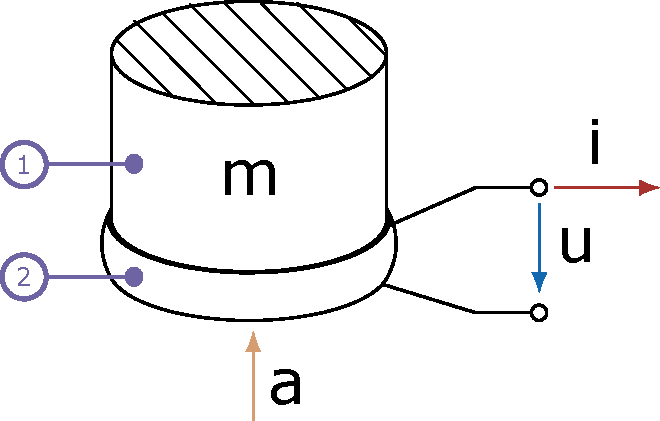
\includegraphics[scale=0.5]{\imgpath/measurement/sensors/piezo_sensor}
    \captionof{figure}[Piezoelectric accelerometer]{Function principle of a piezoelectric accelerometer}
    \label{fig:piezo_sensor}
\end{minipage}
\hspace{4em}
\begin{minipage}[b]{0.3\textwidth}
    \centering
    \footnotesize
    \def\circlabel#1#2{%
        \begin{tikzpicture}[%
            x=1em,y=1ex,
            baseline={([yshift=3] N.south)},
            font={\fontsize{6pt}{6.2pt}\selectfont},
            ]%
            \node[%
                circle, fill=white, draw=#1, line width=1pt,
                inner sep=2pt, minimum size=8pt, align=center,
                ] (N) {#2};
        \end{tikzpicture}
    }
    \begin{tabular}{c@{ :\hskip 0.5em}l}
        \toprule
        \large{a} & Acceleration\\
        \large{m} & Mass\\
        \large{i} & Induced Current\\
        \large{u} & Induced voltage\\
        \large{\circlabel{WesMixL8qual3}{1}} & Seismic mass\\
        \large{\circlabel{WesMixL8qual3}{2}} & Piezoelectric material\\
    \bottomrule
    \end{tabular}
    \normalsize
    \captionof{table}[Legend to piezoelectric accelerometer]{Legend to \figref{fig:piezo_sensor}}
    \label{tab_piezo_sensor}
\end{minipage}
\end{minipage}\\[4ex]

In seismic accelerometers the base of the arrangement is motion. When describing the one dimensional case, one can express non-stationary random vibrations acting on the accelerometer as
\begin{align}
    m\dv[2]{z}{t} &= c\dv{z}{t} + kz = mg\cos\pqty{\theta}-m\dv[2]{x_1}{t}
\end{align}
where
\begin{description}[topsep=0ex, noitemsep]
    \item $m$ is the seismic mass
    \item $z=x_2-x_1$ is the relative motion between the mass and the base
    \item $x_1$ is the displacement of the base
    \item $x_2$ is the displacement of the mass
    \item $\theta$ is the angle between sense axis and gravity
\end{description}
The second-order system expressed in Laplace transform thus takes the form
\begin{align}
    G(s) &= \frac{X(s)}{F(s)} \frac{K}{s^2/\omega_n^2 + 2\zeta s/\omega_n + 1}
\end{align}
where
\begin{description}[topsep=0ex, noitemsep]
    \item $s$ is the Laplace operator
    \item $K=1/k$ is the static sensitivity
    \item $\omega_n=\sqrt{k/m}$ is the undamped frequency in \si{\radian\per\second}
    \item $\zeta=c/2\sqrt{km}$ is the damping ratio
\end{description}
It is obvious that the performance of accelerometers depends on their static sensitivity, the natural frequency and the damping ratio. We want the accelerometer to have a linear transfer function in the range of operation. But namely the damping ratio can distort a measurement when operating an accelerometer near its eigenfrequency, see \figref{fig:seismic_accelerometer_edited}.


\begin{figure}[!htb]
    \centering
    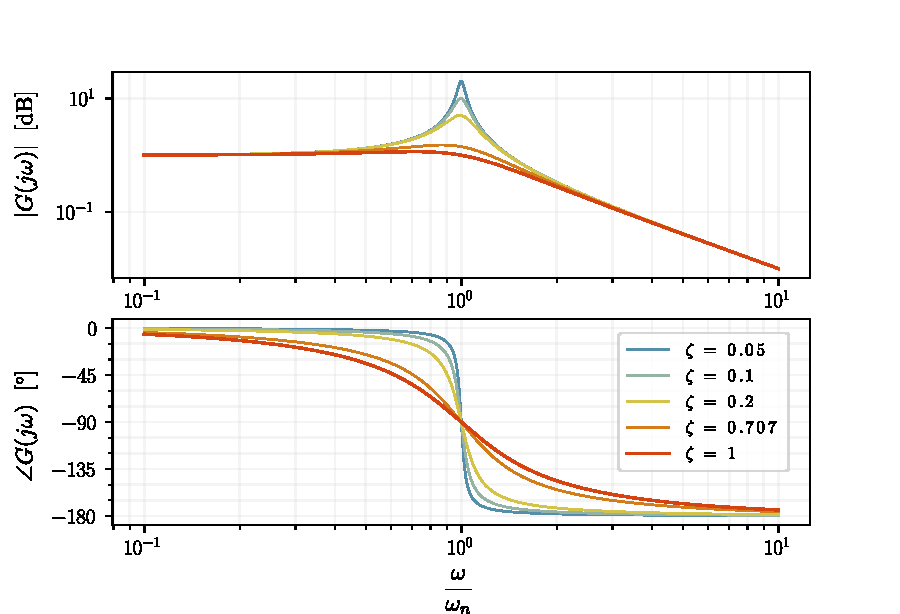
\includegraphics[scale=0.8]{\imgpath/measurement/accel/seismic_accelerometer_edited}
    \caption[Second-Order System Bode plots]{Bode plots of second order system describing the dynamic behavior of seismic accelerometers}
    \label{fig:seismic_accelerometer_edited}
\end{figure}

\subsection{Piezoelectric Sensors}
Some materials develop electric charge proportional to directly applied mechanical stress. The same materials show the converse effect. A proportional strain of the material will occur to an applied electric field.

The first phenomenon has found its application in a variety of self-generating sensors that output electrical signals -- namely in \ac{LC}s and accelerometers, where the piezoelectric charge is converted into a current or voltage signal.

Piezoelectric sensors are designed to exploit the piezoelectric effect of the material in one axis. Additionally, we use amplifier circuits so that the weak electrical signal, induced due to the piezoelectric charge, is elevated to amplitudes that are in the range of operation of standard electronic components. These circuits require additional energy. Commercially available \ac{LC}s therefore require supplied energy -- see \figref{fig:piezo_ampcirc}.

\begin{figure}[!htb]
    \centering
    \subcaptionbox{Piezoelectric sensor connected to a voltage amplifier\label{sfig:piezo_voltage_amp}}{%
        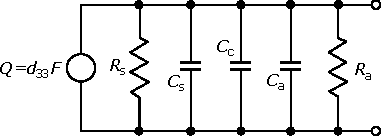
\includegraphics[scale=0.9]{\imgpath/measurement/sensors/piezo_voltage_amp}}
    \hspace{4em}
    \subcaptionbox{Strain gauge in Wheatstone bridge circuit\label{sfig:piezo_current_amp}}{%
        
\includegraphics[scale=0.9]{\imgpath/measurement/sensors/piezo_current_amp}}
    \caption[Piezoelectric sensors in amplifier circuits \cite{webster2018measurement}]{Piezoelectric sensors connected to amplifier circuits \cite{webster2018measurement}}
    \label{fig:piezo_ampcirc}
\end{figure}

Depending on the design of the sensor, piezoelectric materials are used in different shapes. \figref{fig:piezo_designs} shows some possible variations.


\subsection{Strain Gauge Load Cells}

In strain gauge \ac{LC}s the elastic properties of a material probe is exploited.

The probe is loaded in a controlled manner in its elastic region. Deformations are captured by a strain gauge at a suitable location. The probe deformation is directly determined by the force acting on the probe because of Hooke's law.

The strain gauges themselves each use a specific length gauge wire in order to reach a resistance of typically \SI{120}{\ohm}. The wire is bonded between two thin sheets in coiled up form as can be seen in \figref{sfig:strain_gauge}. The sheets act as insulating carrier and can be easily deformed with the intent of passing the load to the wire grid. The gauge is attached to the probe structure by a wax or a resin. The intent is that deformations in transversal direction of the strain gauge act on all coils simultaneously, changing their resistance. By using small sized strain gauges with respect to the probe, the mechanical and thermal properties of the strain gauge become negligible small. As an example, we assume the probe expands. Then a strain gauge on its surface experiences tension. The coils in the grid are therefore stretched and as a result of the generalized Hook's law the coil cross sections decrease. Both the strain in axial direction of the coil and the decreased coil cross sections increase the wire's resistance.

In order to measure deformations one needs to take environmental influences into consideration. It is well known that resistance is susceptible to variations in temperature. Placing the strain gauge in a wheatstone bridge, with resistors, that change their resistance in the same manner as the strain gauge will reduce the influence of temperature significantly -- see \figref{sfig:wheatstone_bridge_single}.

\begin{figure}[!htb]
    \centering
    \subcaptionbox{Strain gauge on structure, with (1) Structure, (2) Metal Pad, (3) Grid and (4) Carrier\label{sfig:strain_gauge}}{%
        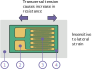
\includegraphics[scale=0.7]{\imgpath/measurement/sensors/strain_gauge}}
    \hspace{4em}
    \subcaptionbox{Strain gauge in Wheatstone bridge circuit\label{sfig:wheatstone_bridge_single}}{%
        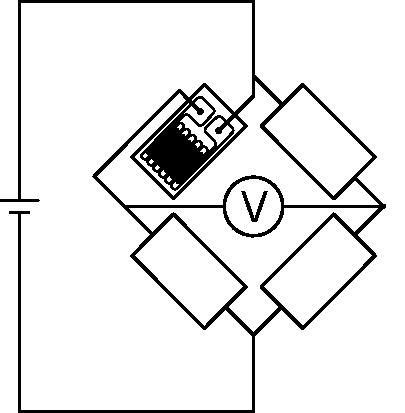
\includegraphics[scale=0.7]{\imgpath/measurement/sensors/wheatstone_bridge_single}}
    \caption[Strain Gauge]{Strain gauge}
    \label{fig:strain_gauge}
\end{figure}

\subsection{Capacitive Accelerometers}

To understand the working principle of capacitive accelerometers, we first consider the displacement sensors.

\subsubsection{Capacitive Displacement Sensors}
The basic sensing element of a displacement sensor typically consists of two parallel electrodes with capacitance C.
\begin{align}
    C &= f(d,A,\varepsilon)
\end{align}

With variable distance, dielectric material or area and with the measurement of the capacitance, we can then deduce the plate displacement in normal and parallel direction to the plates depending on the method used. See \figref{fig:cap_disp} 

In variable displacement sensors, the distance between two capacitive plates is inversely proportional to the capacitance.
\begin{align}
    C(x) &= \frac{\varepsilon A}{x} = \frac{\varepsilon_r\varepsilon_0 A}{x}
\end{align}
where
\begin{description}[topsep=0ex, noitemsep]
    \item $\varepsilon$ is dielectric constant or permittivity
    \item $\varepsilon_r$ is the relative dielectric constant (in air and vacuum $\varepsilon_r\approx 1$)
    \item $\varepsilon_0$ is \SI{8.854188}{\farad\per\meter}, the dielectric constant of vacuum
    \item $x$ is the distance of the plates in \si{\meter}
    \item $A$ is the effective area of the plates in \si{\meter\squared}
\end{description}

In variable area displacement sensors, the capacitance is proportional to the reduction of area due to the movement of the plate.
\begin{align}
   C(x) &= \frac{\varepsilon_r\varepsilon_0\pqty{A-wx}}{d}\label{eqn:var_ar_displace}
\end{align}
where
\begin{description}[topsep=0ex, noitemsep]
    \item $\varepsilon_2$ is the permittivity of the displacing material (e.g. liquid)
    \item $w$ is the width
    \item $wx$ is the reduction in the area due to movement of the plate 
    \item $d$ is the distance of the plates in \si{\meter}
\end{description}

In variable dielectric sensors, the capacitance depends on the ratio of each permittivity in the electric field.
\begin{align}
   C(x) &= \varepsilon_0 w \bqty{\varepsilon_2 l - \pqty{\varepsilon_2-\varepsilon_1}x}\label{eqn:var_diel_displace}\\
\end{align}
where
\begin{description}[topsep=0ex, noitemsep]
    \item $x$ is the displacement normal to the plate's direction
    \item $\varepsilon_1$ is the relative permittivity of the dielectric material
    \item $\varepsilon_2$ is the permittivity of the displacing material (e.g. liquid)
\end{description}
Differential capacitive displacement sensors are setup in capacitive arrangements that aim to eliminate nonlinearities. Different variations of these types of sensors exist. For example we can allow the outer plates to move and fix the middle one or we can reverse this setup. But the range is equal to twice the separation in both cases.

\begin{align}
    2\delta C = C_1-C_2 &= \frac{\varepsilon_r\varepsilon_0 lw}{d-\delta d} - \frac{\varepsilon_r\varepsilon_0 lw}{d+\delta d} = \frac{2\varepsilon_r\varepsilon_0 lwd}{d^2+\delta d^2}\\
    C_1+C_2 &= \frac{\varepsilon_r\varepsilon_0 lw}{d-\delta d} + \frac{\varepsilon_r\varepsilon_0 lw}{d+\delta d} = \frac{2\varepsilon_r\varepsilon_0 lwd}{d^2+\delta d^2}\\
\end{align}
Giving approximately
\begin{align}
    \frac{\delta C}{C} = \frac{\delta d}{d}
\end{align}

\begin{figure}[!htb]
    \sbox0{\subcaptionbox{Variable distance displacement\label{sfig:cap_var_disp}}{%
        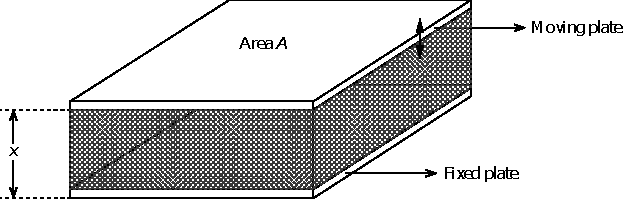
\includegraphics[scale=0.7]{\imgpath/measurement/capac/cap_var_disp}
        }}% a
    \sbox1{\subcaptionbox{Variable area displacement\label{sfig:cap_var_area}}{%
        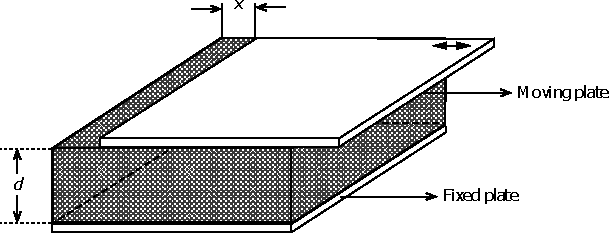
\includegraphics[scale=0.7]{\imgpath/measurement/capac/cap_var_area}
        }}% b
    \sbox2{\subcaptionbox{Variable dielectric displacement\label{sfig:cap_var_diel}}{%
        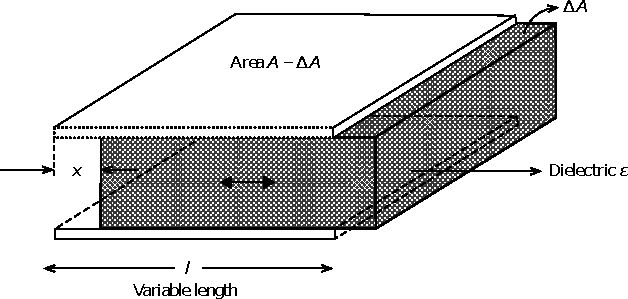
\includegraphics[scale=0.7]{\imgpath/measurement/capac/cap_var_diel}
        }}% c
    \sbox3{\subcaptionbox{Differential capacitive displacement\label{sfig:cap_diff}}{%
        \includegraphics[scale=0.7]{\imgpath/measurement/capac/cap_diff}
        }}% d
    \sbox4{\subcaptionbox{IC smart capacitive displacement \label{sfig:cap_smart}}{%
        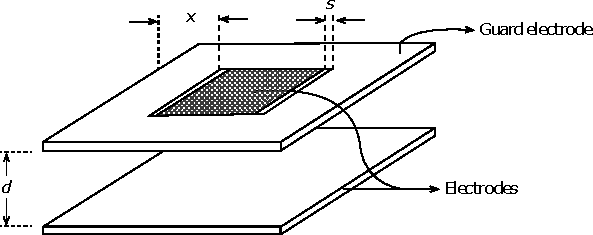
\includegraphics[scale=0.7]{\imgpath/measurement/capac/cap_smart}
        }}% e
    \centering
    {%
        \renewcommand{\arraystretch}{6}%
        \setlength{\tabcolsep}{0em}
        \begin{tabular}{ccc}
            \usebox0 & \usebox1 \\
            \usebox2 & \usebox3 \\
        \end{tabular}%\\[4ex]
        % \usebox4
    }
    \caption[Capacitive displacement sensors]{Capacitive displacement sensors \cite{webster2018measurement}}
    \label{fig:cap_disp}
\end{figure}

\subsubsection{From Displacement to Acceleration}
If one combines a capacitive displacement sensor with a seismic mass, one can use the inertia force to correlate the acceleration to the displacement and hence to the change in the electric field of the sensor. With the use of differential capacitive designs and high machining accuracy these designs can be realized in a tiny form factor as \acf{MEMS}. A scheme of such a sensor is shown in \figref{fig:accelerometer_bent}.

\begin{figure}[!htb]
    \centering
    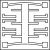
\includegraphics[scale=0.7]{\imgpath/measurement/sensors/accelerometer_bent}
    \caption[Capacitive MEMS Accelerometer]{Capacitive MEMS accelerometer, with acceleration a and the seismic mass m. The bridges attached to the seismic mass act as dielectricum.}
    \label{fig:accelerometer_bent}
\end{figure}

\section{Signal Conditioning and Processing}
In an ideal world, the signal output of a sensor would correlate to the measurand exactly. In real systems this is not the case because of a variety of reasons. In low-frequency applications, the most important ones are:

\begin{itemize}
    \item The voltage or current rating at a sensor's output is not perfectly linear with respect to the measurand. Often the output is pseudo-linear in a limited range of values and deviates from the trajectory for values outside of this range.
    \item Noise and shifts introduced through the inherent impedances of analog components lead to deviations from the voltage or current rating of the sensor as well as deviations of these ratings with respect to the measurand itself.
    \item The quantization process causes the captured value space to have a finite resolution.
    \item Analog signals can only be digitized with a finite sampling rate. A discrete set of data points is captured instead of a continuous signal.
\end{itemize}

The field of signal processing includes analyzing, modifying and synthesizing signals. Most prominently, in data acquisition systems we convert analog signals to digital ones that can be further processed without the parasitic effects of the analog realm. On the opposite side when addressing these parasitic effects one needs to apply signal conditioning. In other words, before every processing step of an analog signal we need to consider signal conditioning. When dealing with digital signals, no signal conditioning is required.

\section{Experimental Modal Analysis}

\ac{EMA} is a powerful tool to detect vibration related problems of mechanical structures. We use modes to characterize resonant vibrations of the system. This section is only a short excerpt of an introduction to \ac{EMA}. An overview has been presented by \citeauthor{schwarz1999experimental} in \cite{schwarz1999experimental}.

\subsubsection{Vibration}

In every vibration one can observe a combination of two different types of vibrations. The forced and the resonant ones. Forced vibrations in a structure are caused by
\begin{itemize}
    \item Internally generated forces
    \item Unbalances
    \item External loads
    \item Ambient excitations
\end{itemize}
Common examples of vibration sources in \ac{MT} are displayed in \figref{fig:vibration_sources}.

\begin{figure}[!htb]
    \centering
    \subcaptionbox{Axis Motion\label{sfig:ball_screw_simple}}{%
        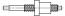
\includegraphics[scale=0.7]{\imgpath/ema/vibration_sources/ball_screw_simple}}
        \hspace{4em}
    \subcaptionbox{Imbalance\label{sfig:imbalance_scheme}}{%
        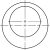
\includegraphics[scale=0.7]{\imgpath/ema/vibration_sources/imbalance_scheme}}
    \hspace{4em}
    \subcaptionbox{Processing Force\label{sfig:processing_force_scheme}}{%
        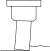
\includegraphics[scale=0.7]{\imgpath/ema/vibration_sources/processing_force_scheme}}
    \\[5ex]
    \begingroup
    \subcaptionbox{Impact Hammer\label{sfig:impulse_hammer_scheme}}[0.5\linewidth]{%
        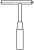
\includegraphics[scale=0.7]{\imgpath/ema/vibration_sources/impulse_hammer_scheme}}
    \endgroup
    \hspace{0em}
    \subcaptionbox{Modal Shaker\label{sfig:modalShaker_scheme}}{%
        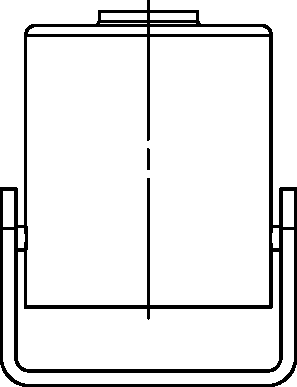
\includegraphics[scale=0.7]{\imgpath/ema/vibration_sources/modalShaker_scheme}}
    \caption[Forced Vibration Sources]{Sources of forced vibration. Note that \subref{sfig:ball_screw_simple}, \subref{sfig:imbalance_scheme} and \subref{sfig:processing_force_scheme} occur during \ac{MT} operation, while \subref{sfig:impulse_hammer_scheme} and \subref{sfig:modalShaker_scheme} are devices that are explicitly used for \ac{EMA} to introduce vibrations into the structure of investigation.}
    \label{fig:vibration_sources}
\end{figure}

Resonant vibration arises when one or more of the natural modes of vibration, inherent properties of the structure under investigation, is excited. Resonant vibration typically amplifies the vibration response to a level that exceeds deflection, stress and strain caused by static loading. 

\subsection{Frequency Response Measurement}

In an \ac{EMA} one needs to determine the \ac{FRF} from input to output. To achieve this we measure the so called response or output function of the structure under investigation. The measurement instrument for this task uses a signal chain in form of \ref{fig:measurement}.
\begin{itemize}
    \item The sensor on the structure translates the physical value (acceleration, velocity or position) into an electrical voltage or current, the analog signal variable.
    \item The amplifier amplifies the typically low power signal to fit it to the input range of the \ac{ADC}.
    \item The \ac{ADC} samples and quantizes the analog signal. It is then converted into a digital signal, in which the quantity is expressed in form of a binary code.
    \item The discrete time signal is then stored on the computer memory.
\end{itemize}

\begin{figure}[!htb]
    \centering
    \includestandalone[width=\linewidth]{\imgpath/ema/measurement/measurement}
    \caption[Frequency Response Measurement]{\ac{FRF} measurement setup}
    \label{fig:measurement}
\end{figure}

\section{Electronic Components}

This section serves as an introduction to the function of selected electronic components and circuits. It does not give a complete overview of the state of the art. For more background on electronics \cite{Stiny2019AeB} and \cite{Tietze2008EC} may be consulted.

Electronic components are divided into two main types; passive and active ones. Where active components are allowed to generate, amplify or oscillate an electrical signal, passive components can only absorb, dissipate or store electric energy.

\subsection{Passive Components}

Because of the increase in digital processing, the number of passive components has decreased drastically in modern electronic circuits. This, in addition to the trend of using more complex devices in favour to multiple simple passive components, has led to a great variety of passive components which are designed with emphasis on reliability.

Typical examples of passive components are:
\begin{description}
    \item[Wires] Depending on the mechanical requirements for the wire, it can either be designed with a solid core or a stranded wire core. A wire consisting of multiple smaller diameter conductors shows better flexibility but reduced current-carrying capacity at the same wire diameter. This is because of the smaller overall conductor cross-section of a stranded wire and, when transmitting high frequency signals, a greater power dissipation due to the more prevalent skin effect. Furthermore the simplicity of solid core wires makes them more resistant to corrosion and more suitable to be used in harsh environments.
    \item[Resistors] Depending on the application different types of resistors can be applied. Fixed value resistors, can be used for safety of other components by dissipating heat or reducing to set the current and voltage in combination relative to other devices. Variable resistors change their value due to different physical phenomena. Thermistors show resistances that are highly susceptible to temperature changes, potentiometers resistance is manually tunable and photoresistors show a light dependant resistance, to name a few. 
    \item[Capacitors] Capacitors store energy in form of an electric field. They have many applications, most prominently in filter circuits and as bypass capacitors to reduce smooth out non constant power draws.
    \item[Inductive Devices] Are devices that store energy in form of an electric field. In modern devices coils are less common due to benefits, when realizing the circuit with capacitors instead. But in specialized applications, namely when converting between electrical and mechanical signals, i.e. in motors, generators, loudspeakers etc.
\end{description}
% \subsubsection{Wires}

% Wires connect several electronic components. Ideally no loss or noise is introduced in wires but inductances occur due to the conductor's shape and material properties as well as electric fields, that are either self induced or present due to ambient conditions.

% Depending on the mechanical requirements for the wire, it can either be designed with a solid core or a stranded wire core. A wire consisting of multiple smaller diameter conductors shows better flexibility but reduced current-carrying capacity at the same wire diameter. This is because of the smaller overall conductor cross-section of a stranded wire and, when transmitting high frequency signals, a greater power dissipation due to the more prevalent skin effect. Furthermore the simplicity of solid core wires makes them more resistant to corrosion and more suitable to be used in harsh environments.

% Braided or foil shielding wires are usually used to shield other wires from ambient fields. Shaped as a tube they enclose one or multiple wires acting as a Faraday cage.

% \subsubsection{Resistors}

% Resistors are loads that reduce the current flow and set the voltage levels within a circuit. There are many different types of resistors.

\subsection{Active Components}
Active components show some form of amplification of the input signal in most cases; in other ones they generate vibrations, but generally an additional energy supply is needed to operate active components.

As an essential example, we consider the \acf{OP-AMP}. The \ac{OP-AMP} is a multi-stage, high gain and galvanically coupled differential amplifier. It is used to amplify an electrical signal, and its function is primarily determined by its surrounding circuit. Namely filters can be realized by using \ac{OP-AMP}s.

Normally \ac{OP-AMP}s are connected to symmetric operating voltages. But when used with digital circuits, a single voltage supply is preferred. For this case, single supply voltage \ac{OP-AMP}s are used. Furthermore, rail-to-rail \ac{OP-AMP}s are have the capability to control the output between the the positive and negative supply voltage.

\begin{figure}[htb!]
    \centering
    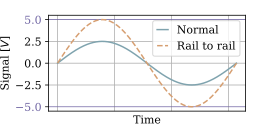
\includegraphics[scale=0.7]{\imgpath/electronics/op_amp/plot_opamp_railrail}
    \caption[OP-AMP controllability]{OP-AMP controllability at $\pm\SI{5}{\volt}$ operating voltage}
    \label{fig:plot_opamp_railrail}
\end{figure}

\subsection{Applictions}
Electrical signal conditioning is based on arrangements of active and passive components in circuits. A good and in depth coverage of active filters and measurement circuits can be found in \cite{Tietze2008EC}. For many common applications a \acf{IC} exists. These circuits internal to chips that come in various package sizes, see \figref{fig:ic_flowchart}.


\subsection{Anti Aliasing Filter}
The \acf{AAF} is used ahead of \ac{ADC}s to reduce the signal bandwidth. More precisely, it aims to reduce the aliasing effect, i.e. the artificial distortion of signals, that occurs when sampling at a finite frequency.

\begin{figure}[!htb]
    \centering
    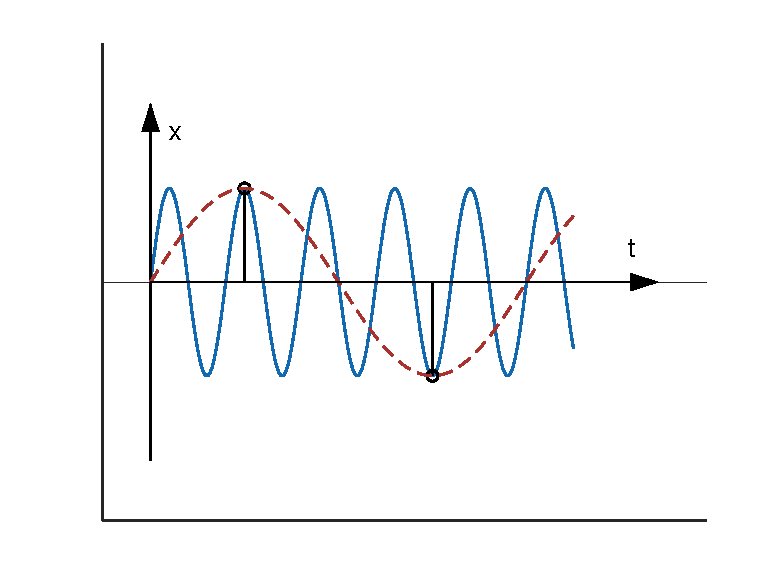
\includegraphics[scale=0.7]{\imgpath/electronics/aaf/plot_aliasing}
    \caption[Aliasing]{Aliasing effect}
    \label{fig:plot_aliasing}
\end{figure}

\subsection{Analog to Digital Converters}

Additionally to other noise sources in the signal chain the \ac{ADC} shows internal noise that can categorized into two uncorrelated main sources. The quantization noise and the thermal noise. The total internal noise can thus be expressed as the Euclidean norm of these two sources.

\begin{align}
    n_\text{ADC} &= \sqrt{n_{\text{ADC},\text{Thermal}}^2 + n_{\text{ADC},\text{Quantization}}^2}
\end{align}

Quantization noise is present due to the process of mapping an infinite number of possible electrical signal values in an analog signal to a finite number of digital codes. Subsequently, any digital output corresponds to an infinite number of analog inputs within range of the output value, plus and minus half the \ac{LSB} size, $s_\text{LBS}$. One can decrease quantization noise by choosing a higher resolution \ac{ADC}.

\begin{align}
    s_\text{LBS} &= \frac{U_{FSR}}{2^m}
\end{align}
where
\begin{description}[topsep=0ex, noitemsep]
    \item $U_{\text{FSR}}$ is the full-scale range of the analog input value and
    \item $m$ is the resolution in number of bits
\end{description}

\begin{figure}[!htb]
    \centering
    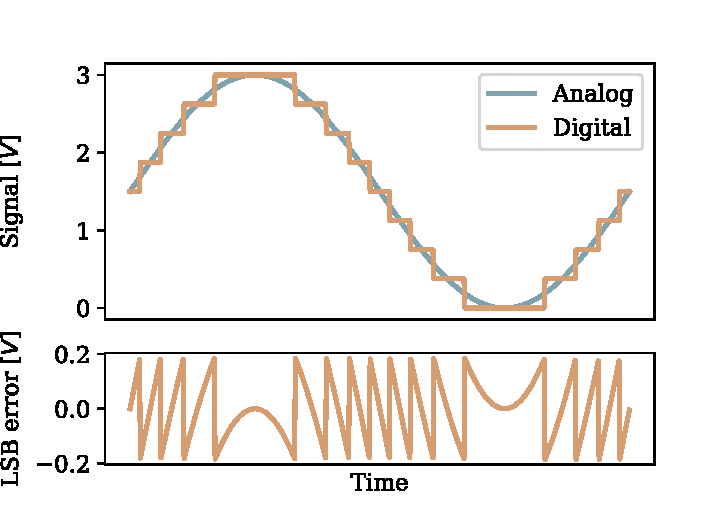
\includegraphics[scale=0.7]{\imgpath/electronics/adc/plot_lsberr}
    \caption[ADC LSB waveform]{\ac{ADC} -- Analog input, digital output and \ac{LSB} error waveform with $s_\text{LBS} = \SI{375}{\milli\volt}$\cite{hall2020fund}}
    \label{fig:plot_lsberr}
\end{figure}

Thermal noise is a phenomenon inherent in all electrical components. Because of this it is a function of the device design and cannot be affected by the embedded system designer. Typically, one assumes the thermal noise to have a Gaussian distribution.

\begin{figure}
    \centering
    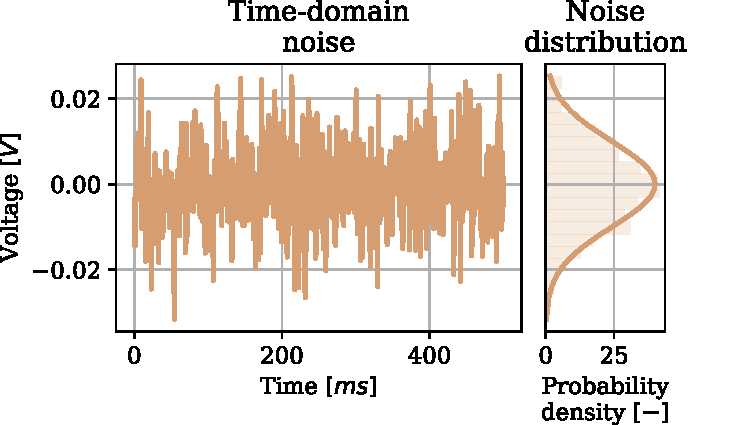
\includegraphics[scale=0.7]{\imgpath/electronics/adc/plot_thermerr}
    \caption[ADC thermal noise]{ADC -- Thermal noise in the time domain with Gaussian probability density \cite{hall2020fund}}
    \label{fig:plot_themerr}
\end{figure}

